\section{Data}

The German electricity market was liberalized in 1998 and is the largest in Europe with a gross production of of 633.2 TWh in 2006 \citep{IEA2007}. More than half of the power is generated with coal, other major sources are nuclear and gas. The German power market is dominated by a few large players (E.ON, RWE, EnBW, Vattenfall). These firms are both transmission system operators and own 90\% of total generation capacity. \cite{Brunekreeft2006} report values for Herfindahl Hirschman Index (HHI)\footnote{This is a common measure of market power and is calculated as sum of the squared market shares in an industry.} of over 2000. Electricity distribution is organized by approximately 900 communal distributors. The German energy market regulator  \emph{Bundesnetzagentur} was installed in 2005. Germany decided on a phase-out of nuclear power generation by 2020. The \emph{German Energy Agency} estimates that investments in generation capacity of up to 40,000 MW will be necessary, see Fig. \ref{fig:nuclear}.

\begin{figure}[htb]
  \centering
\caption{Estimated nuclear power capacity, 2007 to 2023}
  \includegraphics[width=.7\textwidth]{germandata/nuclear.pdf}
  \label{fig:nuclear}
\\
 \scriptsize Source: \cite{IEA2007a}
\end{figure}

The capacities of the four major electricity generators can be found in Tab. \ref{tab:majorcapacities}.

\begin{table}[htb]
\centering
\scriptsize
\caption{Installed capacities in MW of major players in Germany}

\begin{tabular}[htb]{crrrrrrrrr}
\hline
           &      Hydro &    Nuclear &  Soft coal &  Hard coal &        Gas &        Oil &     Pumped \\
\hline\hline
       RWE &        741 &       5499 &      10554 &       7249 &       4297 &        188 &        793 \\

      E.ON &       1320 &       8473 &       1425 &       9461 &       3808 &       1779 &       1110 \\

Vattenfall &          9 &       1421 &       6932 &       1729 &        870 &       1429 &       2883 \\

      EnBW &        447 &       4272 &        453 &       3288 &       1083 &        617 &        368 \\
\hline
\end{tabular} 
\label{tab:majorcapacities}
\\
\scriptsize Source: \cite{Ellersdorfer2005}
\end{table}

Figure \ref{fig:investcosts} contains investment costs for different technologies.

\begin{figure}[htb]
  \centering
\caption{Levelised costs for generation units starting commercial operation in 2015}
  \includegraphics[width=.5\textwidth]{germandata/investmentcosts.pdf}
  \label{fig:investcosts}
\\
 \scriptsize Source: \cite{IEA2007c}
\end{figure}

The major stake of electricity trading is done in OTC markets for which it is hard to obtain data. Exchange prices from the EEX can be used as a good approximation. We see the expected positive relationship when comparing the exchange prices to the actual electrcity demand per hour.

\begin{figure}[htb]
  \centering
\caption{Price-quantity relationship}
  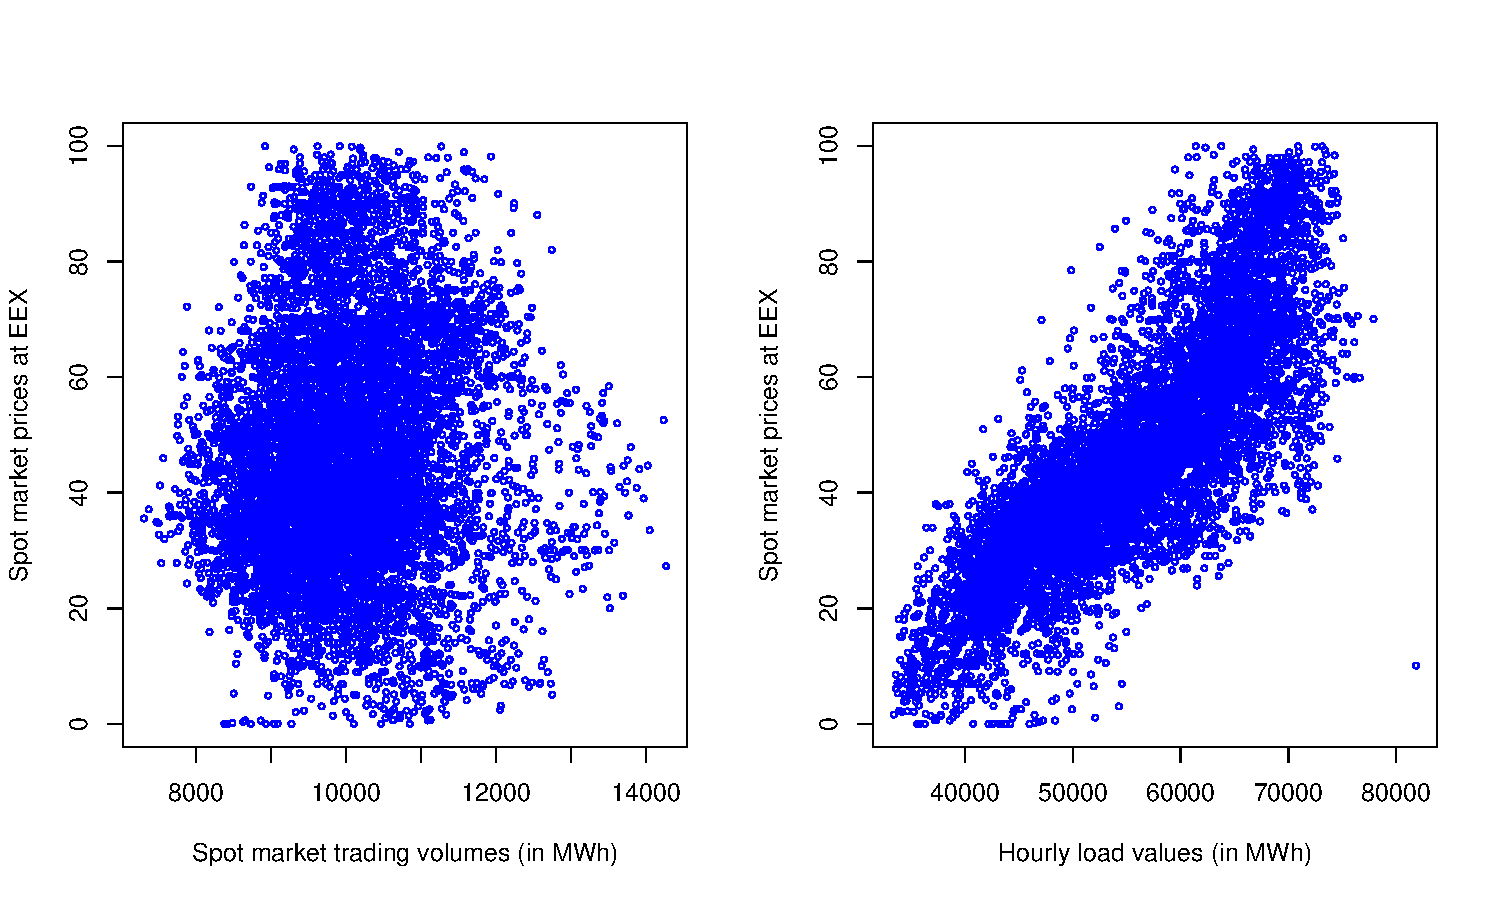
\includegraphics[width=.8\textwidth]{germandata/pricequant.pdf}
  \label{fig:investcosts}
\\
 \scriptsize Source: EEX, UCTE
\end{figure}

\clearpage

%%% Local Variables: 
%%% mode: latex
%%% TeX-master: "../emarket_simulation"
%%% End: 
